%%%%%%%%%%%%%%%%% PREAMBLE %%%%%%%%%%%%%%%%%%%%%%%%%%%%
\documentclass[aspectratio=169]{beamer}
%\documentclass[handout,aspectratio=169]{beamer} % turns on handout mode to surpress the \pause
\usepackage{xcolor}
\usepackage{colortbl} 
\usetheme[progressbar=frametitle]{metropolis}
\usepackage{changepage}
\usepackage{pgfpages}
\usepackage{booktabs}
\usepackage{bm}
\usepackage{threeparttable}
\usepackage{caption}
\usepackage{subfig}
\usepackage{natbib}
\usepackage{transparent}
\setbeamercovered{transparent} 


% turn off/on showing notes in the presentation
%\setbeameroption{show notes on second screen}
\setbeameroption{hide notes}
\setbeamertemplate{note page}[plain]

\definecolor{BlueGreen}{cmyk}{0.755,0,0.33,0}
\definecolor{RawSienna}{cmyk}{0,0.72,1,0.45}


\hypersetup{
    colorlinks=true,
    linkcolor= blue,
    urlcolor= blue,
    citecolor=blue
}
\usepackage{graphicx}
\usepackage{hyperref}

% metropolis theme
\usetheme[progressbar=frametitle]{metropolis}


%Changes the page numbers - {arabic}= arabic numerals, {gobble}=no page numbers, {roman}=Roman numerals
\pagenumbering{arabic}

\newcommand{\source}[1]{\caption*{\tiny Source: {#1}} }


\begin{document}

\title{New Results}
\date{\today}

\maketitle

\begin{frame}{Infiltration with different levels of aggregation
}
\begin{figure}
    \centering
    \includegraphics[width=\linewidth]{output_clean/figures/inf_aggregation.png}
    \label{fig:placeholder}
\end{figure}
\end{frame}

\section{Updated Main Figures}


\begin{frame}{Infiltration - minus decomposition
}
\begin{figure}
    \centering
    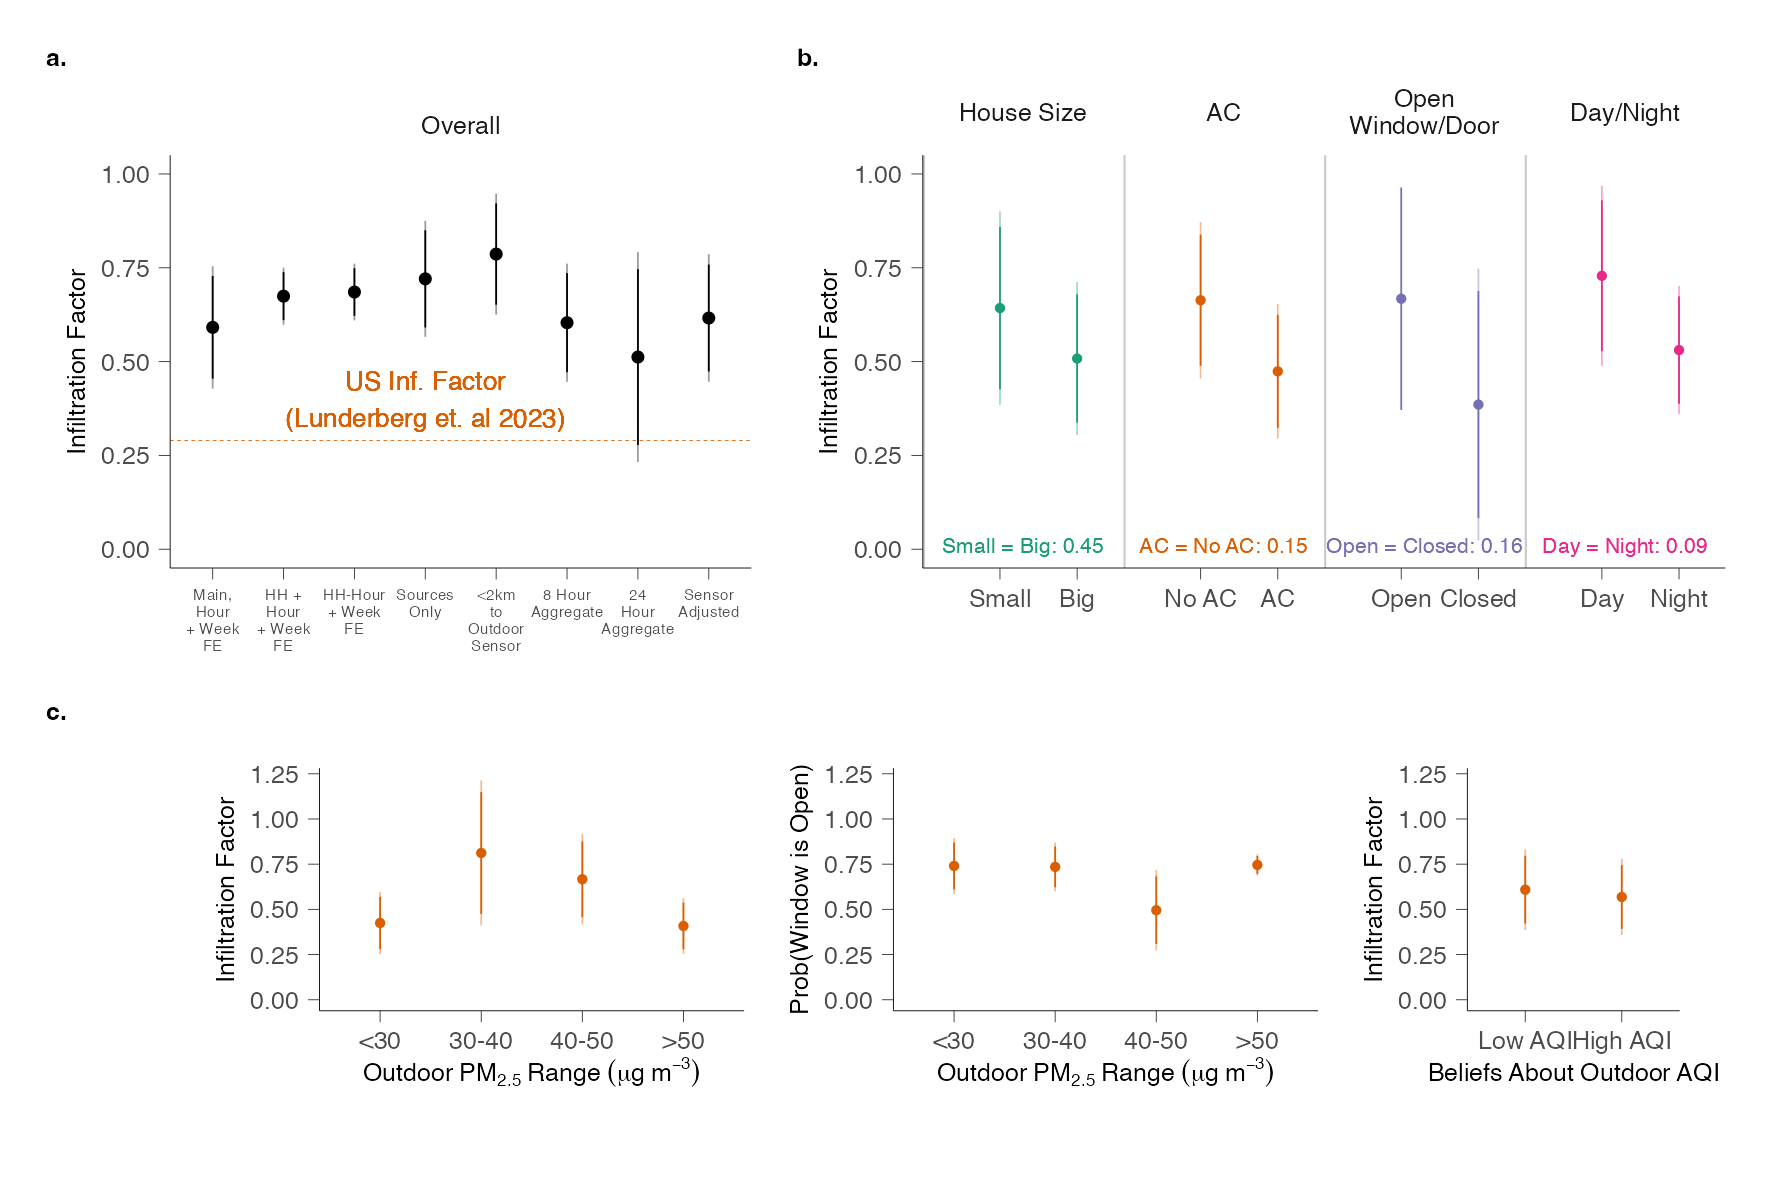
\includegraphics[width=.7\linewidth]{output_clean/figures/fig2_infiltation.png}
\end{figure}
\end{frame}

\begin{frame}{Decomposition methodology}
\scriptsize
    To quantify the contribution of observable pollution sources to indoor PM$_{2.5}$, we estimate the following panel specification:
\begin{align}
\label{eq:decomp_main}
    PM^{\text{indoor}}_{it}
=&
\beta_1 PM^{\text{outdoor}}_{it}
+\beta_2 \text{Smoke}_{i}
+\beta_3 \text{WasteBurn}_{i} 
+\beta_4 \text{KitchenSource}_{i}
+\beta_5 \text{Cooking}_{i} \\
\notag
&+\beta_6 \text{DistPrimary}_{i}
+\alpha_h+\delta_w+\varepsilon_{it}
\end{align}

where $i$ indexes household-monitor observations and $t$ indexes time. We include hour-of-day fixed effects ($\alpha_h$) and week fixed effects ($\delta_w$), and cluster standard errors at the respondent and date-hour levels.

For each source $j$, we compute its mean contribution to indoor PM$_{2.5}$ as
\begin{align*}
\label{eq:mean_contrib}
\overline{C}_j = \hat{\beta}_j \cdot \overline{X}_j,
\end{align*}
where $\overline{X}_j$ is the sample mean of source $j$. We then express this in share terms:
\begin{align*}
\label{eq:share_contrib}
\text{Share}_j = \frac{\overline{C}_j}{\overline{PM^{\text{indoor}}}}.
\end{align*}
This ``effect size $\times$ prevalence/intensity'' construction directly maps to the reviewer’s suggested accounting identity. We report 95\% confidence intervals by propagating coefficient confidence bounds through the first equation above.
\end{frame}



\begin{frame}{Decomposition of sources}
\begin{figure}
    \centering
    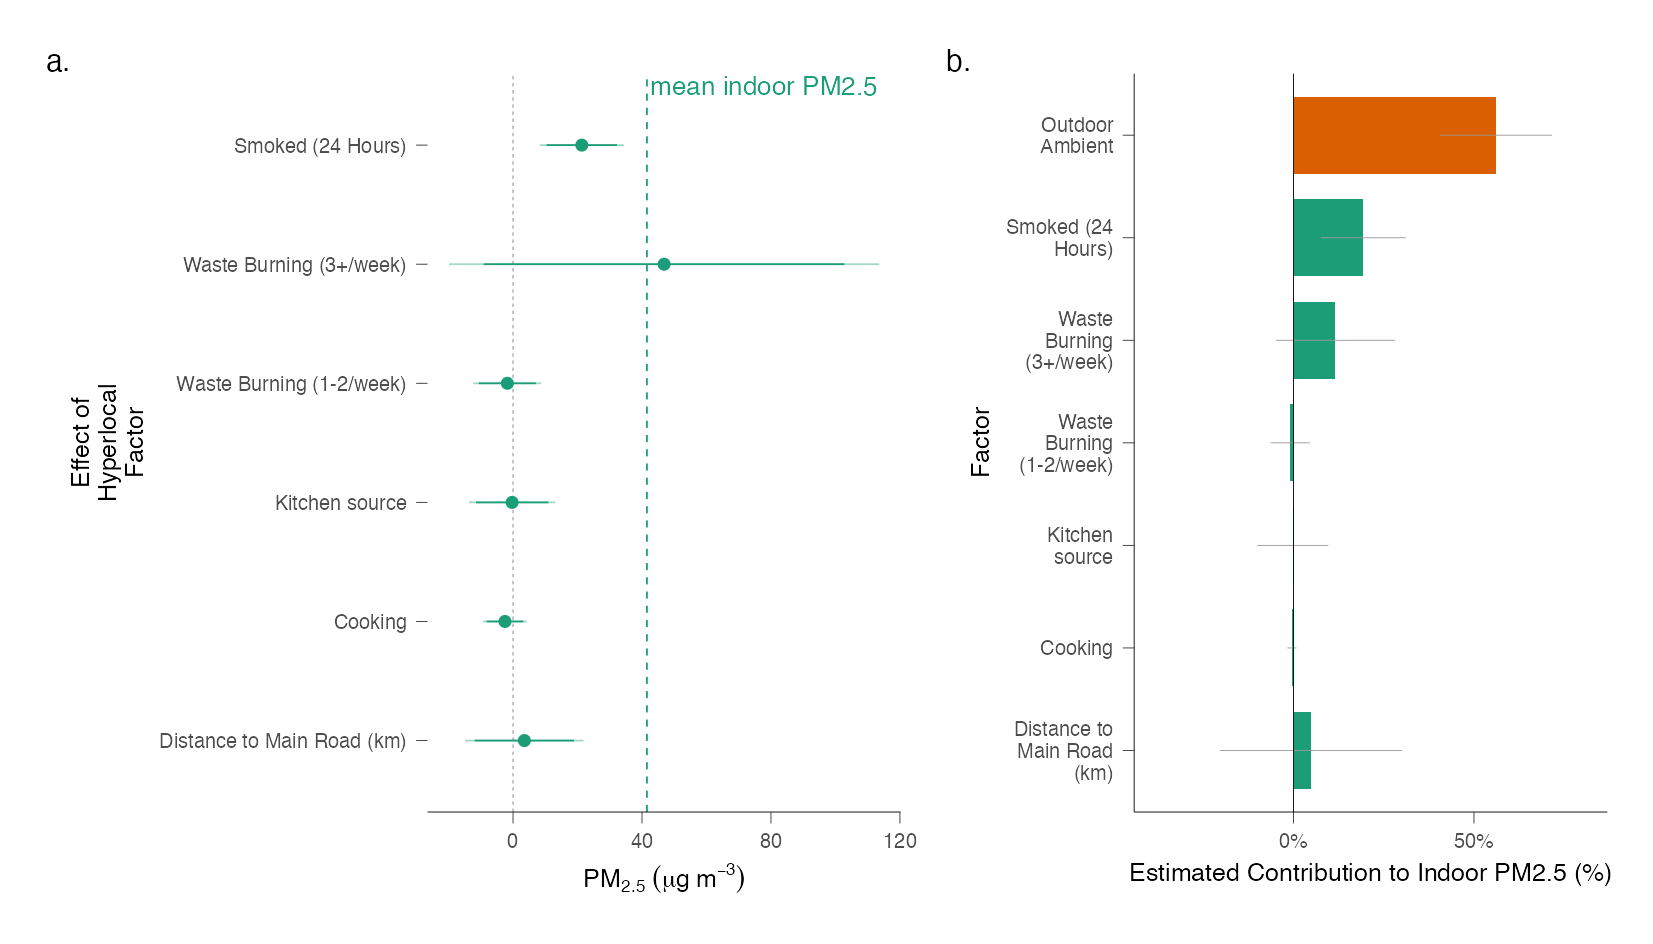
\includegraphics[width=.5\linewidth]{output_clean/figures/fig3_sources.png}
\end{figure}
\end{frame}


\begin{frame}{Variance decomposition (complementary).}
\scriptsize
To complement mean contributions, we compute LMG relative-importance shares. This provides each source’s contribution to explained variance ($R^2$), which we report alongside mean-contribution shares.

\end{frame}

\begin{frame}{Appendix - Contribution to Mean $PM_{2.5}$
}
\begin{table}[!h]
  \centering
  \resizebox{\textwidth}{!}{%
    \begin{threeparttable}
      \caption{Contribution to mean indoor pm}
      
\begin{tabular}{cccccc}
\toprule
Source & Reg. Estimate & p.value & Mean Value of Source & Mean Contribution & $R^2$ Contribution\\
\midrule
Outdoor Ambient & 0.59 & 0.000 & 39.41 & 56\% & 33\%\\
Smoked (24 Hours) & 21.33 & 0.001 & 0.38 & 19\% & 23\%\\
Kitchen source & -0.28 & 0.968 & 0.31 & 0\% & 0\%\\
Cooking & -2.49 & 0.469 & 0.08 & 0\% & 0\%\\
Distance to Main Road (km) & 3.52 & 0.707 & 0.57 & 5\% & 0\%\\
\addlinespace
Waste Burning (1-2/week) & -1.76 & 0.743 & 0.21 & -1\% & \\
Waste Burning (3+/week) & 46.85 & 0.168 & 0.10 & 12\% & \\
\bottomrule
\end{tabular}

      \begin{tablenotes}
        \footnotesize
        \item \textit{Notes:}
      \end{tablenotes}
    \end{threeparttable}
  }%
\end{table}

\end{frame}


\begin{frame}{Appendix - Contribution to Pollution Spikes
}
\begin{table}[!h]
  \centering
  \resizebox{\textwidth}{!}{%
    \begin{threeparttable}
      \caption{Contribution to indoor spikes}
      
\begin{tabular}{cccccc}
\toprule
Source & Reg. Estimate & p.value & Mean Value of Source & Mean Contribution & $R^2$ Contribution\\
\midrule
Outdoor Ambient & 0.000 & 0.008 & 39.41 & 28\% & 2\%\\
Smoking Household & 0.032 & 0.000 & 0.38 & 57\% & 54\%\\
Kitchen source & -0.006 & 0.180 & 0.31 & -9\% & 2\%\\
Cooking & 0.008 & 0.191 & 0.08 & 3\% & 1\%\\
Distance to Main Road (km) & -0.006 & 0.109 & 0.57 & -16\% & 5\%\\
\addlinespace
Waste Burning (1-2/week) & -0.002 & 0.663 & 0.21 & -2\% & \\
Waste Burning (3+/week) & 0.047 & 0.164 & 0.10 & 23\% & \\
 &  &  &  &  & 19\%\\
\bottomrule
\end{tabular}

      \begin{tablenotes}
        \footnotesize
        \item \textit{Notes:}
      \end{tablenotes}
    \end{threeparttable}
  }%
\end{table}

\end{frame}

\begin{frame}{Appendix - Density of Distance to Roads}
\begin{figure}
    \centering
    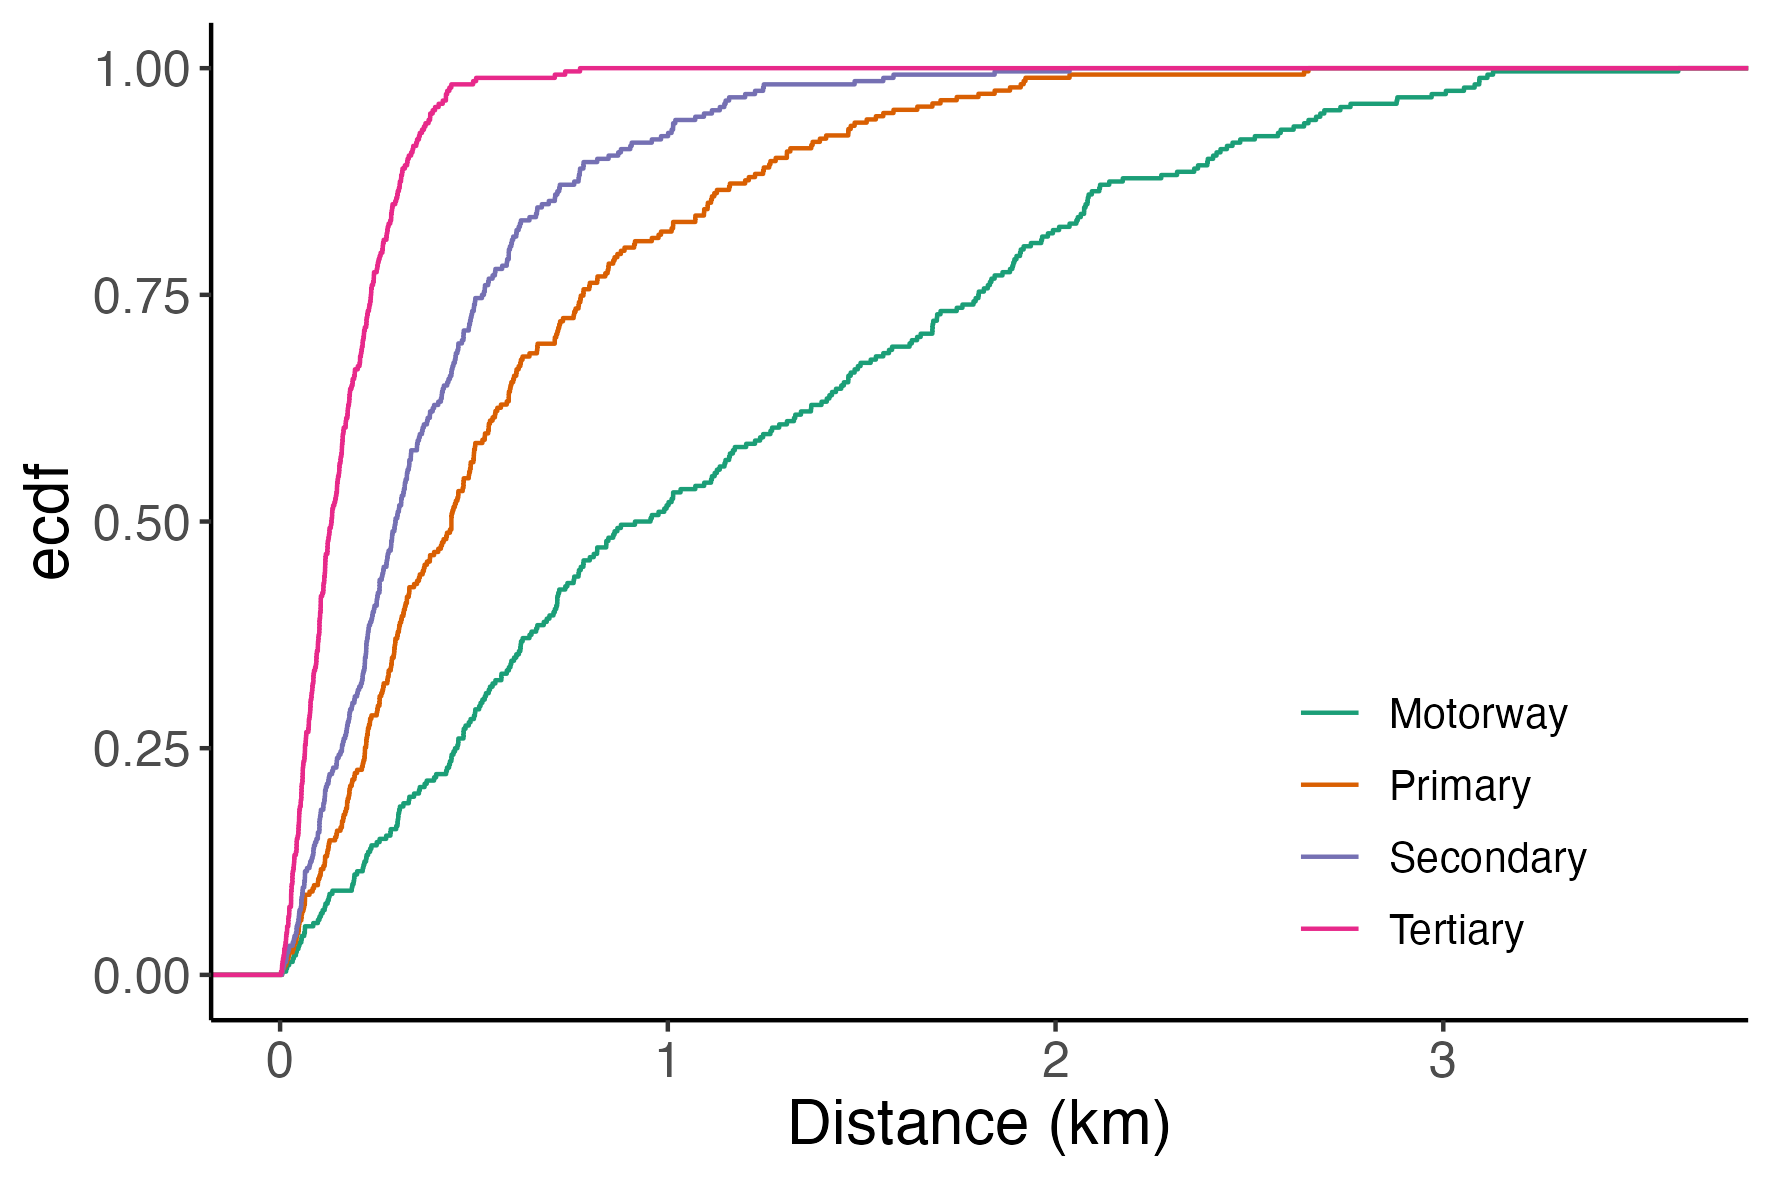
\includegraphics[width=.8\linewidth]{output_clean/figures/distance_to_road_ecdf.png}
\end{figure}
\end{frame}

\begin{frame}{Decomposition by Income}
\scriptsize 
We re-estimate Equation~\eqref{eq:decomp_main} separately by income quartile $q$. Let $\overline{PM}^{\text{indoor}}_q$ denote mean indoor PM$_{2.5}$ in quartile $q$, and let $\overline{C}_{j,q}$ denote quartile-specific source contributions. The unexplained residual is:
\begin{equation}
\label{eq:other_term}
\text{Other}_q
=
\overline{PM}^{\text{indoor}}_q
-
\sum_{j \in \mathcal{J}_{\text{identified}}}\overline{C}_{j,q}.
\end{equation}
In practice, because ambient outdoor PM and smoking are the most precisely estimated across quartiles, we define:
\begin{equation}
\text{Other}_q
=
\overline{PM}^{\text{indoor}}_q
-
\left(
\overline{C}_{\text{outdoor},q}
+
\overline{C}_{\text{smoking},q}
\right).
\end{equation}
This residual captures cooking, other indoor sources, and hyperlocal outdoor sources not separately identified with sufficient precision.
\end{frame}
\begin{frame}{Decomposition by Income}
\begin{figure}
    \centering
    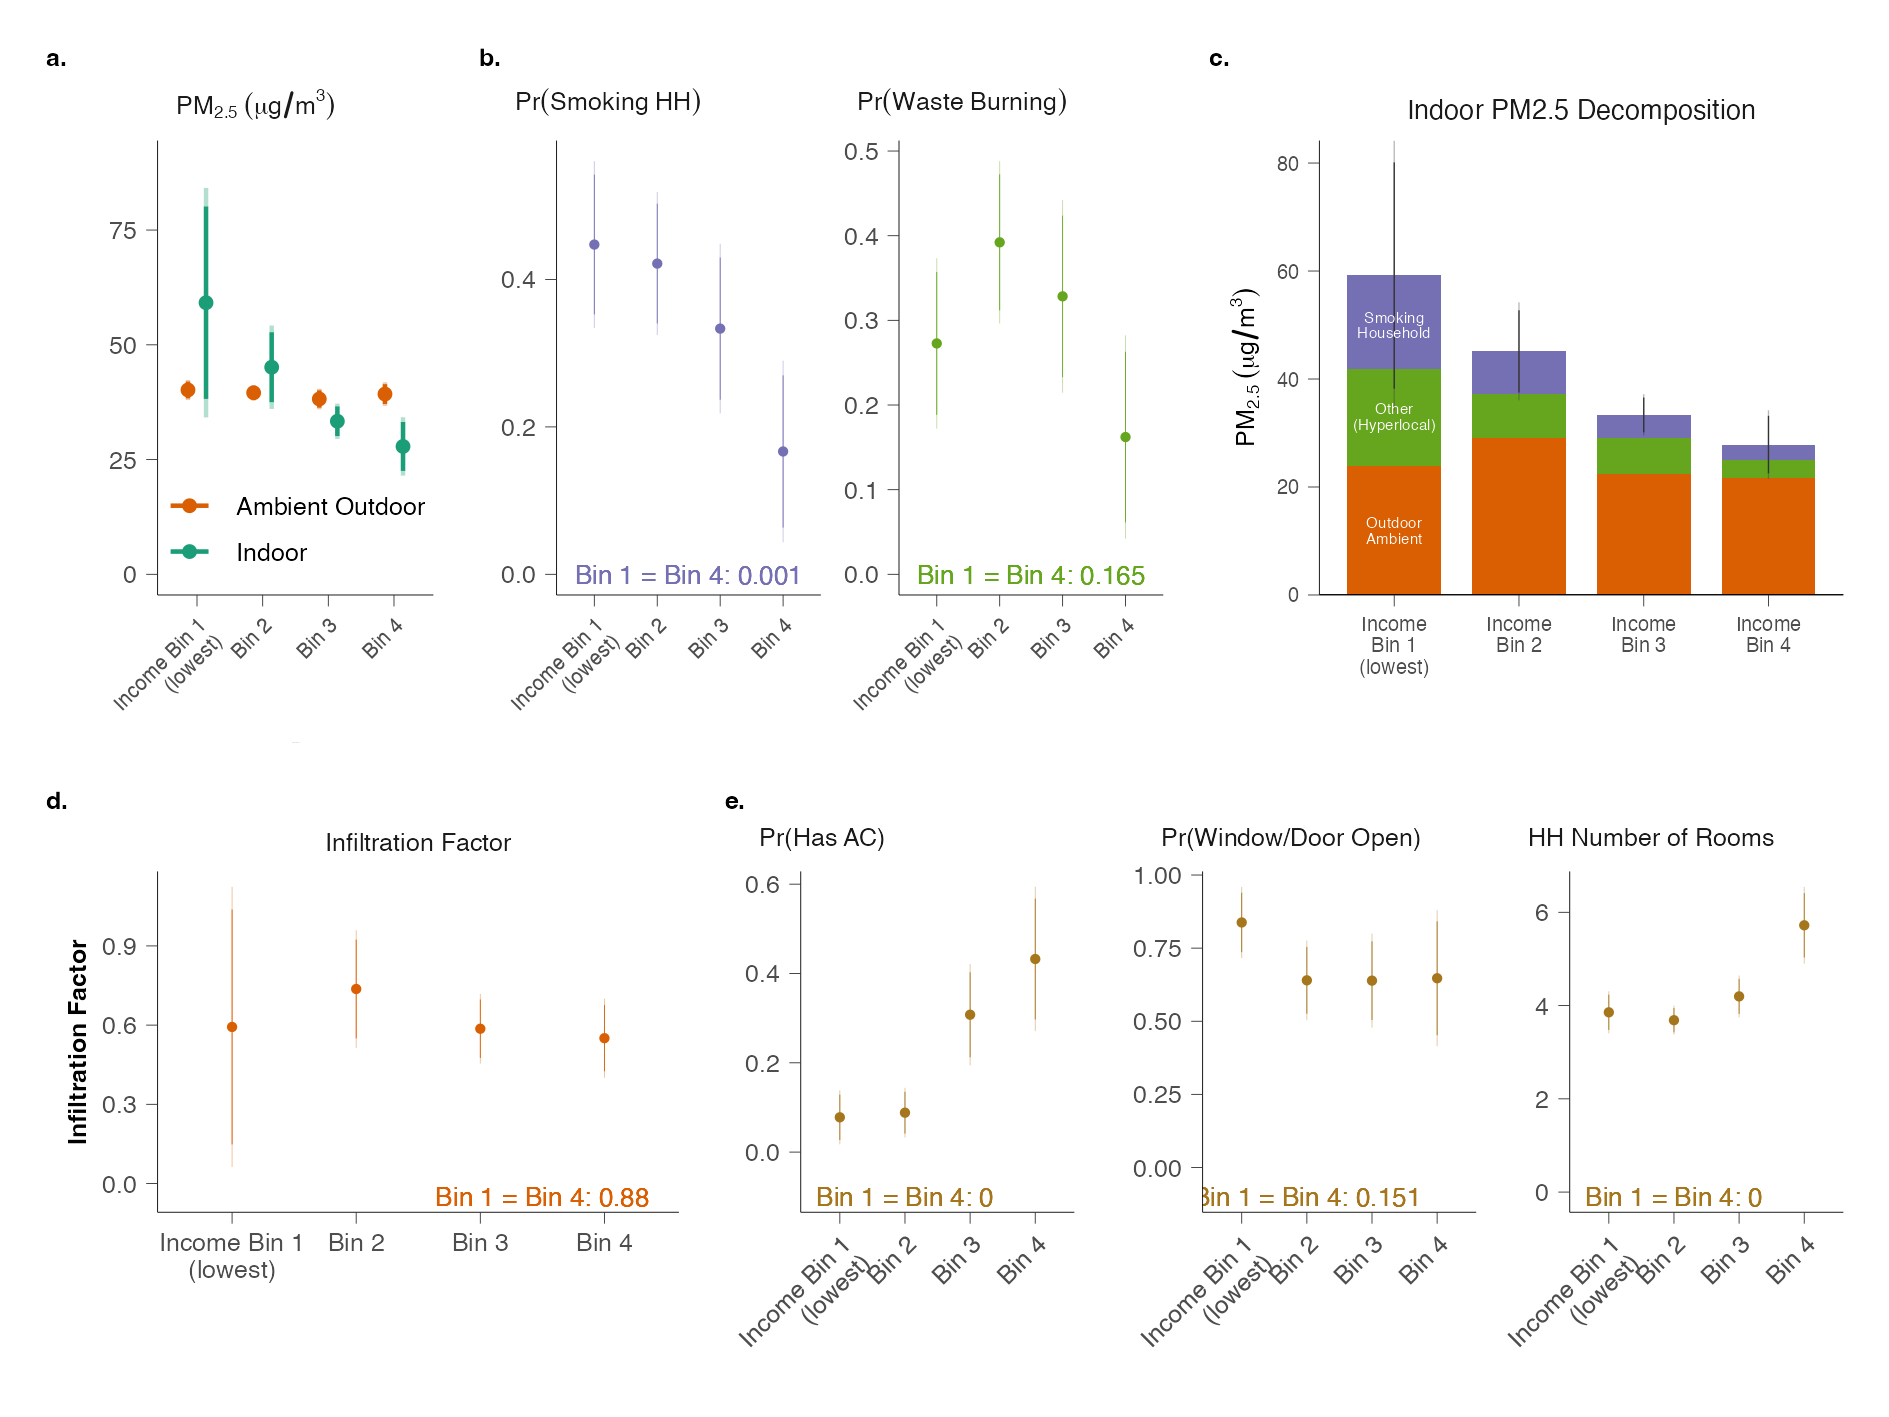
\includegraphics[width=.8\linewidth]{output_clean/figures/fig4_pm_income.png}
\end{figure}
\end{frame}

\begin{frame}{Appendix: correlation between outdoor ambient and waste burning}
\begin{table}[!h]
  \centering
  \resizebox{.5\textwidth}{!}{%
    \begin{threeparttable}
      \caption{Correlation - outdoor ambient and waste burning}
      
\begin{tabular}{lcc}
   \toprule
   Dependent Variable: & \multicolumn{2}{c}{Outdoor PM2.5}\\
                            & Closest 3 Sensors & HH Within 2km of Outdoor Sensor \\   
   Model:                   & (1)               & (2)\\  
   \midrule
   \emph{Variables}\\
   Waste Burning (1-2/week) & 0.570             & 0.431\\   
                            & (0.779)           & (0.770)\\   
   Waste Burning (3+/week)  & 4.06$^{***}$      & 5.12$^{***}$\\   
                            & (1.06)            & (1.79)\\   
   Outdoor Temperature      & -0.351            & 0.182\\   
                            & (0.248)           & (0.260)\\   
   Outdoor Humidity         & -0.182$^{***}$    & -0.164$^{***}$\\   
                            & (0.043)           & (0.048)\\   
   \midrule
   \emph{Fixed-effects}\\
   Week FE                  & Yes               & Yes\\  
   Hour FE                  & Yes               & Yes\\  
   \midrule
   \emph{Fit statistics}\\
   Observations             & 759,777           & 394,345\\  
   R$^2$                    & 0.38432           & 0.37470\\  
   Within R$^2$             & 0.00992           & 0.01250\\  
   \bottomrule
\end{tabular}



      \begin{tablenotes}
        \footnotesize
        \item \textit{Notes:}
      \end{tablenotes}
    \end{threeparttable}
  }%
\end{table}
\end{frame}


\end{document}